\section{Rudin Chapter 11}

\subsection{Poisson Integral}

The Poisson kernel is
\[
P_{r}(t)=\sum_{n=-\infty}^{\infty} r^{\lvert n \rvert }e^{ int }\qquad 0\leq r<1, t\text{ real}
\]
If $z=re^{ i\theta }$,
\begin{equation}
P_{r}(\theta-t)=\mathrm{Re}\left[ \frac{e^{ it }+z}{e^{ it }-z} \right]=\frac{1-r^2}{1-2r\cos(\theta-t)+r^2}
\label{7f4037}
\end{equation}
\[
\frac{1}{2\pi}\int_{-\pi}^{\pi} P_{r}(t) \, \mathrm{d}t=1
\]
From \cref{7f4037} ,we have $P_{r}(t)>0$, $P_{r}(t)=P_{r}(-t)$, $P_{r}(t)<P_{r}(\delta)$, for $0<\delta<\lvert t \rvert\leq\pi$. Then
\[
\lim_{ r \to 1 } P_{r}(\delta)=0\qquad 0<\delta\leq \pi
\]
Now denote $B_1(0)$ by $U$, $\partial B_1(0)$ by $T$. Indentify the spaces $L^{p}(T)$ and $C(T)$ with the corresponding spaces of $2\pi$ -period functions in $\mathbb{R}^{1}$.

Regard $P_{r}(\theta-t)$ as $P(z=re^{ i\theta },e^{ it })$, then
\[
P(z,e^{ it })=\frac{1-\lvert z \rvert ^2}{\lvert e^{ it }-z \rvert ^2}\qquad z\in U,e^{ it }\in T
\]
The Poisson integral $P[f]$ is
\[
F(re^{ i\theta })=(P_{r}*f)(\theta)=\frac{1}{2\pi}\int_{-\pi}^{\pi} P_{r}(\theta-t)f(t) \, \mathrm{d}t\qquad f\in L^{1}(T)
\]
If $f$ is real,
\[
P[f]=\mathrm{Re}\left[ \frac{1}{2\pi}\int_{-\pi}^{\pi} \frac{e^{ it }+z}{e^{ it }-z}f(t) \, \mathrm{d}t  \right]=\mathrm{Re}\underbrace{ \left[ \int_{X}^{} \frac{\mathrm{d}\mu(t)}{\varphi(t)-z}  \right] }_{ \underset{ \text{since }\varphi(X)\cap D=\varnothing }{ \in H(D)\text{ by Theorem 10.7} } }\text{ is harmonic.}
\]
$f=u+iv$, then $P[f]=P[u]+iP[v]$ is harmonic.

Poisson integrals of continuous function \underline{behave well} near the boundary of $U$.
\begin{figure}[H]
\centering
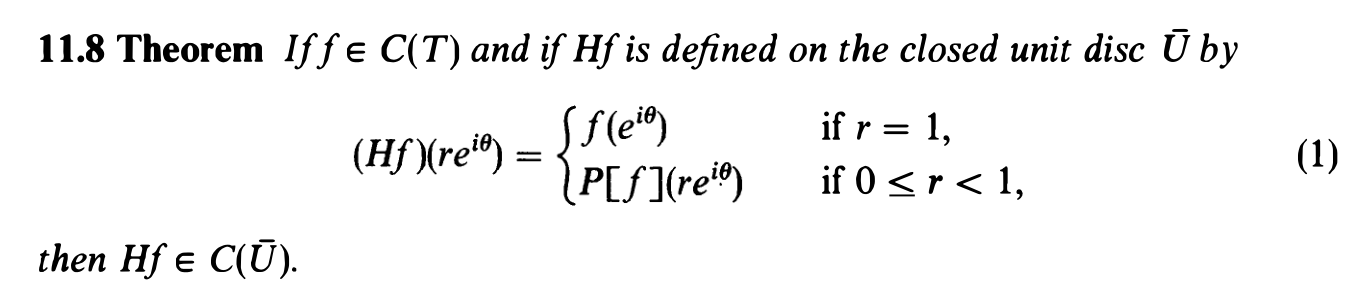
\includegraphics[width=\textwidth]{rudin-harmonic-function-2025052210.png}
% \caption{}
\label{}
\end{figure}

\begin{note}
This theorem, using Poisson integral, solves the boundary value problem\footnote{the Dirichlet problem}: given $f\in C(T)$, find \underline{harmonic} $F$ in $U$.
\end{note}
The harmonic $F$ is also unique.
\begin{figure}[H]
\centering
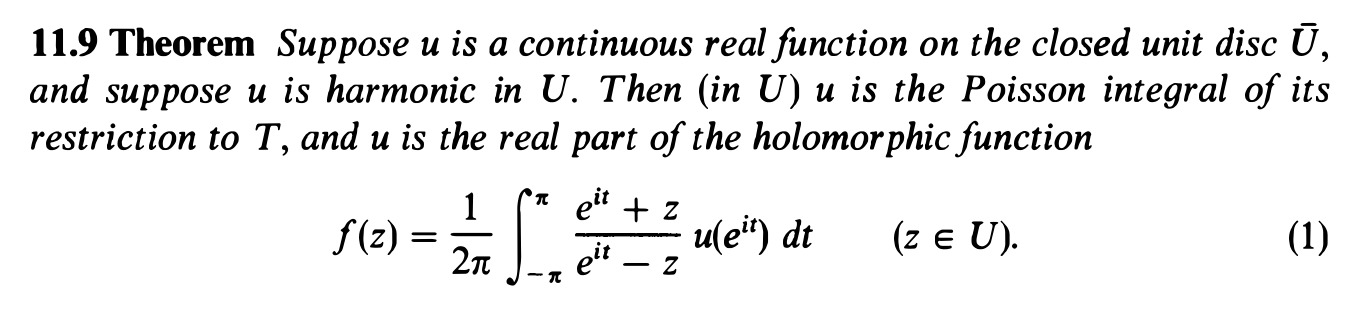
\includegraphics[width=\textwidth]{rudin-harmonic-function-2025052211.png}
% \caption{}
\label{}
\end{figure}

\begin{proof}
By theorem 10.7, $f\in H(D)$. Let $u_1=\mathrm{Re}f$, $u_1$ is harmonic. NTS: $h\coloneqq u-u_1\equiv0$ on $U$. Assume not, WLOG, $\exists z_0\in U$, s.t. $h(z_0)>0$; pick $0<\epsilon<h(z_0)$, $g\coloneqq h+\epsilon \lvert z \rvert ^2$, then $g|_{T}=\epsilon<h(z_0)<g(z_0)$. As $\Delta g=4\epsilon>0$, $g$ is subharmonic, by maximum principle, this is a contradiction.
\end{proof}

For harmonic\footnote{in $U$.} $u\in H(\overline{U})$,
\[
u(z)=\frac{1}{2\pi}\int_{-\pi}^{\pi} \underbrace{ \mathrm{Re}\left[ \frac{e^{ it }+z}{e^{ it }-z} \right] }_{ =P_{r}(\theta-t)= \frac{1-r^2}{1-2r\cos(\theta-t)+r^2}}u(e^{ it }) \, \mathrm{d}t\qquad z\in U
\]
For $B_{R}(a)$, by \cref{7f4037},
\begin{equation}
u(a+re^{ i\theta })=\frac{1}{2\pi}\int_{-\pi}^{\pi} \frac{R^2-r^2}{R^2-2Rr\cos(\theta-t)+r^2}u(a+R e^{ it }) \, \mathrm{d}t
\label{9f27a7}
\end{equation}

Let $u$ harmonic in open $\Omega$. For $\overline{B_R(a)}\subset \Omega$, $u$ satisfies \cref{9f27a7} \footnote{ \cref{9f27a7} is the criterion of harmonic function, due to the above two theorems.}, and $u=\mathrm{Re}f$ for some $f\in H(B_{R}(a))$, where $f$ is unique up to $+i\cdot\text{const.}$

The Poisson integral also yields information about sequences of harmonic functions.
\begin{figure}[H]
\centering
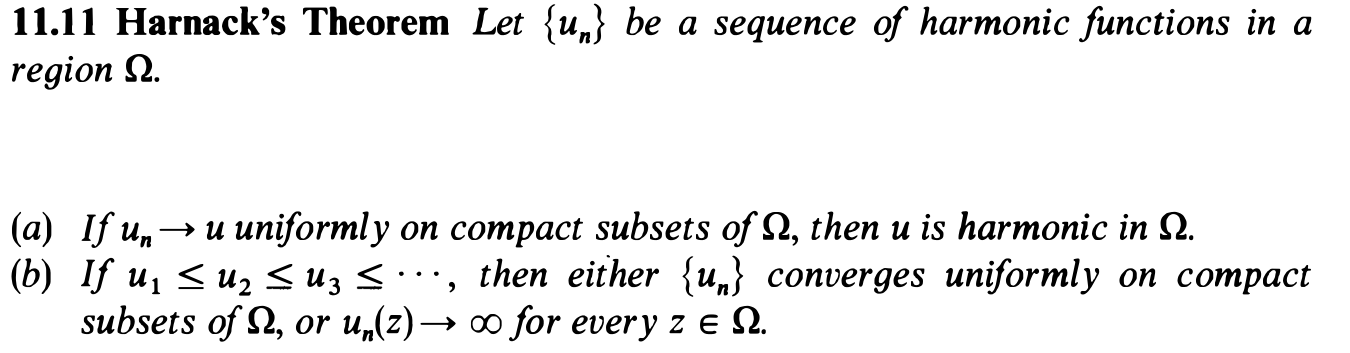
\includegraphics[width=\textwidth]{1-rudin-harmonic-function-2025052211.png}
% \caption{}
\label{}
\end{figure}

\begin{proof}
(a) As $u_n\rightrightarrows u$ on $\overline{B_{R}(a)}\subset \Omega$, $u_n$ satisfies \cref{9f27a7}, we have $u$ satisfies  \cref{9f27a7}, thus $u$ is harmonic.

(b) Assume that $u_1\geq0$, $u\coloneqq \sup u_n$, $A\coloneqq \{ x:u(x)<\infty \}$, $B\coloneqq\Omega-A$. For any $B_{r}(a)\subset A$,
\[
\frac{R-r}{R+r}\leq \frac{R^2-r^2}{R^2-2Rr\cos(\theta-t)+r^2}\leq \frac{R+r}{R-r}
\]
\[
u_n(a+re^{ i\theta })=\frac{1}{2\pi}\int_{-\pi}^{\pi}  \frac{R^2-r^2}{R^2-2Rr\cos(\theta-t)+r^2}u_n(a+R e^{ it }) \, \mathrm{d}t \leq\frac{R+r}{R-r}\cdot\underbrace{ \frac{1}{2\pi}\int_{-p}^{\pi} u_n(a+R e^{ it }) \, \mathrm{d}t }_{ =u_n(a+0\cdot e^{ i\theta })=u(a) }  
\]
Thus
\begin{equation}
\frac{R-r}{R+r}u_n(a)\leq u_n(a+re^{ i\theta })\leq \frac{R+r}{R-r}u_n(a)
\label{ae7692}
\end{equation}

Let $n\to \infty$, then \cref{ae7692} also holds for $u$. Thus $A,B$ are open. As $\Omega$ is connected, $A=\varnothing$ or $\Omega$. We are done!
\end{proof}

\subsection{Schwarz reflection principle}

\begin{figure}[H]
\centering
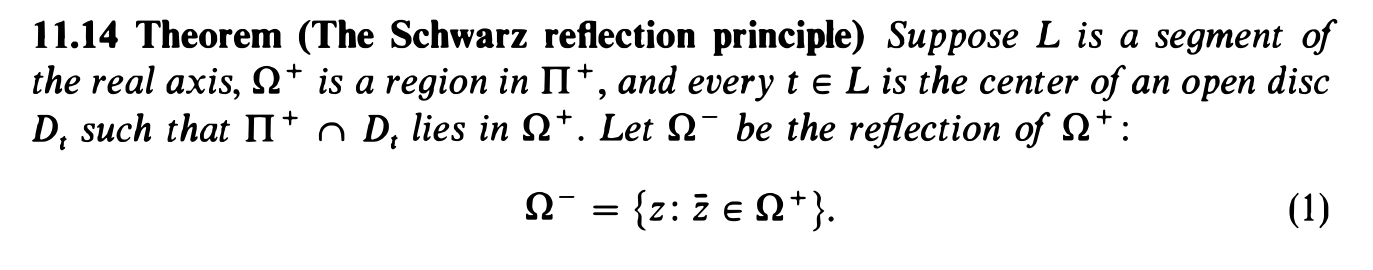
\includegraphics[width=\textwidth]{2-rudin-harmonic-function-2025052212.png}
% \caption{}
\label{}
\end{figure}
\begin{figure}[H]
\centering
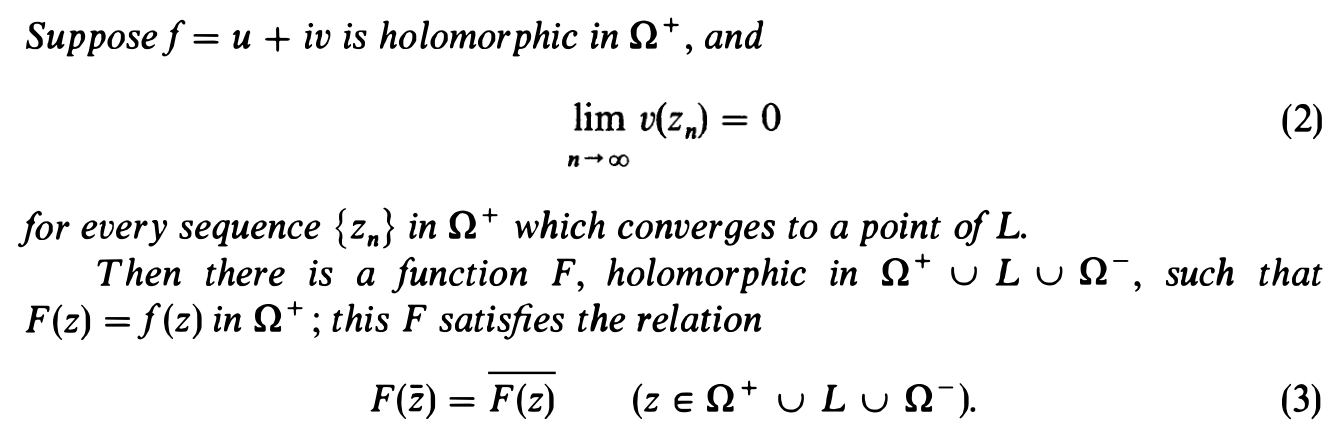
\includegraphics[width=\textwidth]{3-rudin-harmonic-function-2025052212.png}
% \caption{}
\label{}
\end{figure}

The theorem asserts $f\in H(\Omega^{+})$ can be extended to $F\in H(\Omega)$, where $\Omega\coloneqq\Omega^{+}\cup L\cup \Omega^{-}$. $f=u+i v$, we extend $v$ to $\Omega$ by letting $\left.v\right|_{L}=0$, and $\left.v\right|_{\Omega^{-}}(z)=\overline{v(\overline{z})}$.

\subsection{Boundary Behavior of Poisson Integrals}

Let $u_{r}(e^{ i\theta })\coloneqq u(re^{ i\theta })$, $0\leq r<1$. Theorem 11.8 can be restated as: for $f\in C(T)$, $F=P[f]$, then $F_{r}\rightrightarrows f$ on $T$ as $r\to 1$. i.e. $\lim_{ r \to 1 }\lVert F_{r}-f \rVert_{\infty}=0$.

We replace $L^{\infty}$ by $L^{p}$:
\begin{figure}[H]
\centering
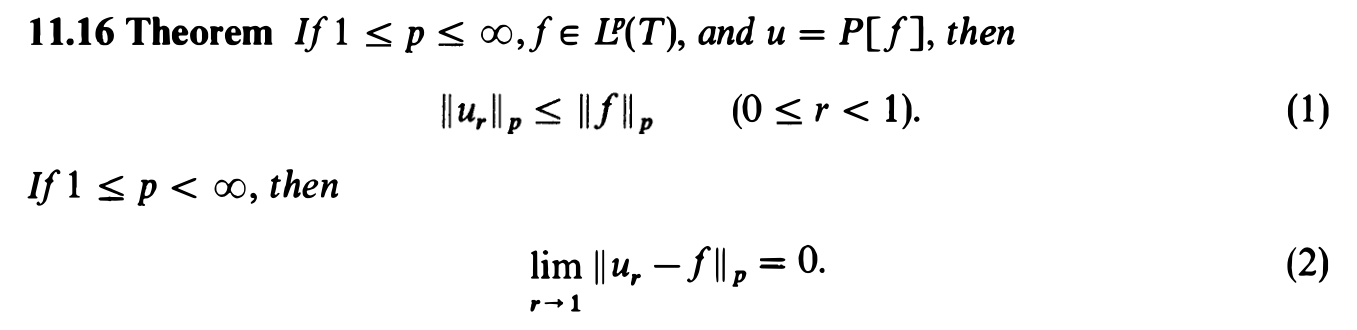
\includegraphics[width=\textwidth]{4-rudin-harmonic-function-2025052212.png}
% \caption{}
\label{}
\end{figure}

\begin{proof}
\[
u_{r}(e^{ i\theta })=\frac{1}{2\pi}\int_{-\pi}^{\pi} f(t)P_{r}(\theta-t) \, \mathrm{d}x \eqqcolon \int_{X}f(t)d\mu
\]
Then
\[
\lvert u_{r}(e^{ i\theta }) \rvert ^{p}=\left\lvert  \int_{X}^{} f(t) \, \mathrm{d}\mu   \right\rvert ^{p}\leq \left( \int_{X}^{} \lvert f(t) \rvert  \, \mathrm{d}\mu \right)^{p}\leq \int_{X}^{} \lvert f(t) \rvert ^{p} \, \mathrm{d}x\cdot \underbrace{ \int_{X}^{} 1^{p} \, \mathrm{d}\mu }_{ =1 }  =\frac{1}{2\pi}\int_{-\pi}^{\pi} \lvert f(t) \rvert ^{p}P_{r}(\theta-t) \, \mathrm{d}t
\]
Integrate $\theta$ ove $[-\pi,\pi]$, then we obtain (1).

As $C(T)$ is dense in $L^{p}(T)$ for $1\leq p<\infty$ \footnote{$\overline{C(T)}^{L^{\infty}(T)}\subsetneq L^{\infty}(T)$}, pick $g\in C(T)$ s.t. $\lVert f-g \rVert_{p}<\epsilon$, $v\coloneqq P[g]$, then
\[
\lVert u_{r}-f \rVert_{p} \leq \underbrace{ \lVert u_{r}-v_{r} \rVert_{p} }_{ =\lVert (u-v)_{r} \rVert _{p}\leq \lVert g-f \rVert _{p}<\epsilon } +\underbrace{ \lVert v_{r}-g \rVert _{p} }_{ \leq \lVert v_{r}-g \rVert _{\infty} }+\underbrace{ \lVert g-f \rVert _{p} }_{ <\epsilon }\leq 2\epsilon+\lVert v_{r}-g \rVert _{\infty}
\]
By theorem 11.8, $\lVert v_{r}-g \rVert_{\infty}\to0$, therefore $\lVert u_{r}-f \rVert_{p}\to 0$ as $r\to1$.
\end{proof}

\subsection{The representation theorem}

\begin{figure}[H]
\centering
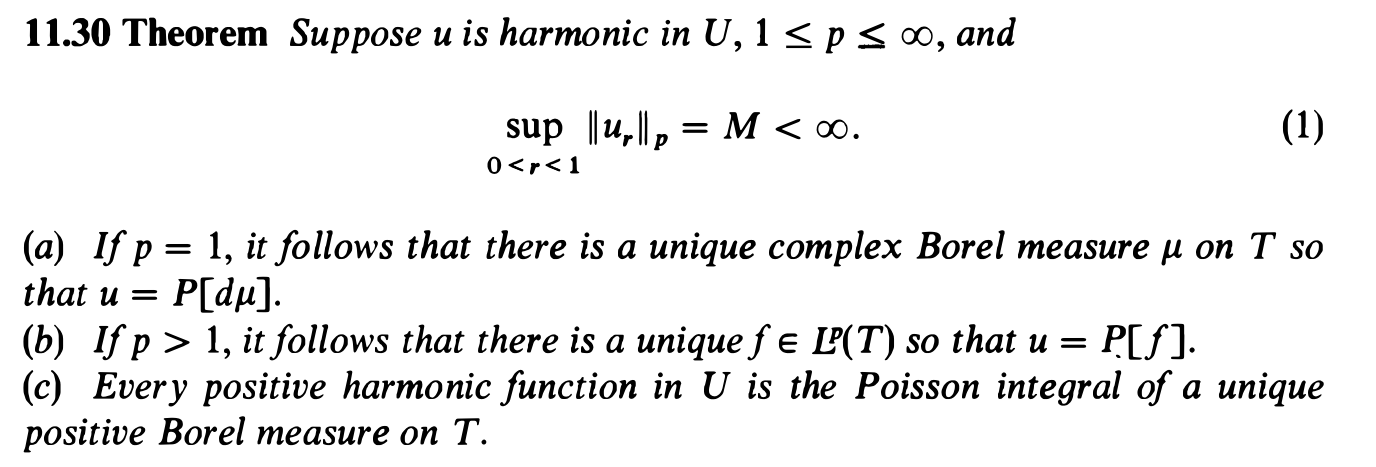
\includegraphics[width=\textwidth]{8-rudin-harmonic-function-2025052212.png}
% \caption{}
\label{}
\end{figure}

\subsubsection{\texorpdfstring{$H^{\infty}$}{H^infty} space}

\begin{figure}[H]
\centering
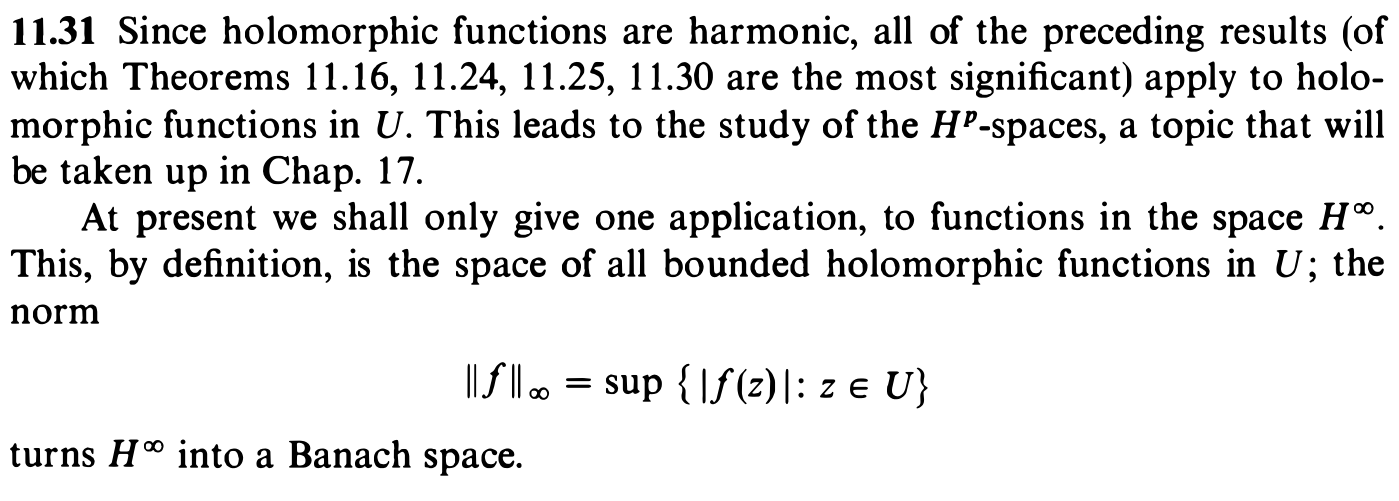
\includegraphics[width=\textwidth]{6-rudin-harmonic-function-2025052212.png}
% \caption{}
\label{}
\end{figure}

\begin{figure}[H]
\centering
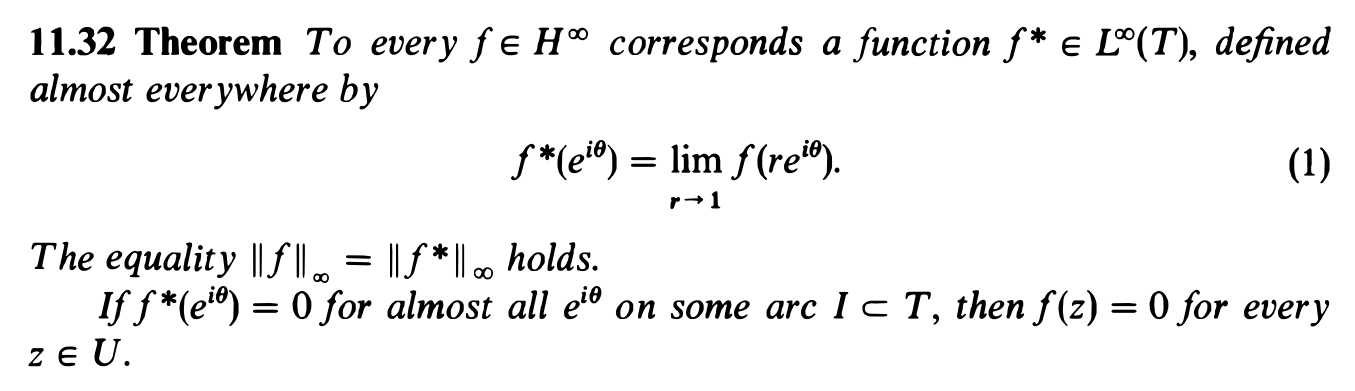
\includegraphics[width=\textwidth]{7-rudin-harmonic-function-2025052212.png}
% \caption{}
\label{}
\end{figure}

A considerably stronger uniqueness theorem will be obtained later.
